\documentclass[11pt]{article}
\usepackage{float}
\usepackage{graphicx}
\usepackage{tabularx}
\usepackage{adjustbox}
\usepackage{amsmath,amssymb,trimclip,adjustbox}
\usepackage{textcomp}
\begin{document}
	\begin{titlepage}
		\begin{center}
			\Large{Warsaw University of Technology's}\\
			\Large{Faculty of Mathematics and Information Science}\\
			[0.3in]
			\begin{figure}[H]
				\centering
				
\includegraphics[width=0.4\linewidth, height=0.25\textheight]{./media/uni_logo.jpeg}
				\label{Figure:f04}
			\end{figure}
			\Large{\bfseries Knowledge Representation and Reasoning}\\
			[0.3in]
			\Large{\bfseries Project number 2:}\\
			\Large{\bfseries Deterministic Action With Cost}\\
			\Large{\bfseries Supervisor: Dr Anna Radzikowska}\\
			[0.3in]
			\textsc{\Large{Created By}\\
				Rishabh Jain,
				Rahul Tomar,
				Kuldeep Shankar,\\ 
				Alaa Abboushi,
				Haran Dev Murugan,\\
				Bui Tuan Anh.\\}
		\end{center}	
	\end{titlepage}
	\tableofcontents
	\newpage
	\section{Introduction}\label{sec:intro}
	Let C2 be a class of dynamic systems satisfying the following assumptions:
	\begin{enumerate}
		\item Inertia law
		\item Complete information about all actions and fluent. 
		\item Only Determinism
		\item Only sequential actions are allowed.
		\item Characterizations of actions:\begin{itemize}
			\item Precondition represented by set of literals(a fluent or its negation);if a precondition does not hold, the action is executed but with empty effect
			\item Postcondition (effect of an action) represented by a set of literals.
			\item Cost $k \in N $ of an action, actions with empty effects cost 0. Each action has a fixed cost, if it leads to non-empty effects. 
		\end{itemize}
		\item Effects of an action depends on the state where the action starts.
		\item All actions are performed in all states.
		\item Partial description of any state of the system are allowed.
		\item No constraints are defined.	 
	\end{enumerate}
	\section{Scenario}\label{sec:scenario}
	A. Can a given program:
	\begin{itemize}
		\item always
		\item ever
	\end{itemize} 
	be executed during at most cost units? \\
	B. Does a given condition \(\alpha\) hold 
	\begin{itemize}
		\item always
		\item ever
	\end{itemize}
	after performing a given program in an initial state?\\ 
	C. Is the Cost k enough to realize the given program?
	\section{Syntax}\label{sec:syntax}
	A system is defined by a set of fluent {\bfseries F}, actions {\bfseries Ac} and Cost {\bfseries k \(\in\) N} and characterized by signature {\bfseries(F, Ac, k)}\\
	A formula is any propositional combination of fluent:
	
	$\alpha$ :: $\neg\alpha$ \textbar $\alpha\wedge\beta$ \textbar $\alpha\vee\beta$ \textbar $\alpha\rightarrow\beta$\\ 
	The system and changes occurring within can be described through a sequence of statements defined in the table:
	\begin{table}[h]
		\centering
			\begin{tabular}{|p{2cm}|p{3cm}|p{8cm}|}
				\hline
				\bfseries Statement & \bfseries Format & \bfseries Description\\
				\hline
				Initial Statement & initially \(\alpha\) & Initial condition \(\alpha\) of the fluent \\
				\hline
				Effect Statement & Ac costing k causes \(\alpha\) & Perform action Ac for cost k in any state leads to the effect \(\alpha\).\\
				\hline	
				Release Statement & Ac costing k causes \(\alpha\) & Perform action Ac for cost k in any state might, but need not, change the value of \(\alpha\).\\
				\hline
				Constraint Statement & Always \(\alpha\) & Every state satisfies condition \(\alpha\).\\
				\hline
				%Fluent Specification Statement & & \\	
				%\hline	
				Value Statement & \(\alpha\) after A1....An & The condition \(\alpha\) always (must) hold after performing the sequence A1 ….An of actions.\\
				\hline
				Observation Statement & observable \(\alpha\) after A1 ….An & The condition \(\alpha\) sometimes (may) holds after performing the sequence A1 ….An of actions.\\
				\hline
			\end{tabular}
		\caption{Sequence of Statements}
		\label{tab:table01}
	\end{table}
	\section{Semantics}
	Let D be an action domain of the class AQ. A structure for a language L:\par
	S = ($  \Sigma  $ , $ \sigma $ 0, k) where;\par
	\begin{itemize}
		\item $  \Sigma  $  is non empty set of states.\par
		
		\item $ \sigma $ 0 $ \in $  $ \sum $ is an initial state
	\end{itemize}\par
	$ \sum $  is the transition function dependent on any possible states satisfying $ \sigma $  $ \in $  $  \Sigma  $ , as well as any\par
	actions A $ \in $  Ac performed in cost k $ \in $  N.\par
	\begin{itemize}
		\item k: Ac $ \rightarrow $  N
	\end{itemize}\par
	As is expected, any action A $ \in $  Ac and in any state $ \sigma $  $ \in $  $  \Sigma  $ , Additionally:\par
	\begin{itemize}
		\item $  \Sigma  $  is an array of states fulfilling any constraints.
	\end{itemize}\par
	Now, consider action domain D. For a structure S = ($ \sum $ , $ \sigma $ 0, k),\par
	a partial mapping $ \psi $ s : Ac$\ast \times \sum \rightarrow $  2\par
	$ \sum $  is defined as:\par
	\begin{itemize}
		\item $ \psi $ s($ \sum $ , $ \sigma $ , k) = $ \sigma $ \par
		
		\item If $ \psi $ s is defined for 1 n performed at state $ \sigma $  for cost k $ \in $  N, then $ \psi $ s(( 1 n-1), $ \sigma $ , k) .
	\end{itemize}\par
	For D being the action domain and S = ($ \sum $ , $ \sigma $ 0, k) being a structure for AQ it can be stated that:\par
	\begin{itemize}
		\item A fluent f $ \in $  F if inertial in D iff (non-inertial f) $ \notin $  D.\par
		
		\item A value statement ($ \alpha $  after 1 n for cost k) is true in S iff $ \psi $ s(( 1 n-1), $ \sigma $ , k) $\vDash$  $ \alpha $  for every $ \psi $ s previously defined.\par
		
		\item An observation Statement (observable $ \alpha $  after 1 n for cost k) is true in D iff $ \psi $ s(( 1 n-1), $ \sigma $ ,k) $\vDash$  $ \alpha $  for some $ \psi $ s previously defined.\par
	\end{itemize}
	$ \sum $  for every A $ \in $  Ac, k $ \in $  N and $ \sigma $  $ \in $  $ \sum $  is:\par
	for all $\sigma$ , $\sigma$ \textquoteright $\in$  $\sum$ and for every A $\in$ Ac, k $\in$ N assume New (A, $ \sigma $ , $ \sigma $ \textquoteright, t\textquoteright) is a set of all literals such\par
	that $ \sigma $ \textquoteright $\vDash$  and:\par
	\begin{itemize}
		\item f is inertial (f $ \in $  F) and $ \sigma $ (f) $ \neq $  $ \sigma $ \textquoteright(f), or\par
		
		\item For some statement (A releases f) $ \in $  D it holds $ \sigma $ 
	\end{itemize}\par
	\subsection{Denote:}
	\begin{enumerate}
		\item = the action domain obtained from D by removing all constraint statements.\par
		
		\item Mod( ) = the set of all models = ($  \Sigma  $ , , ) of in the sense of AR.\par
		
		\item Mod$\ast$ ( ) = the set of all model S = ($  \Sigma  $ , 0) $ \in $  Mod( ) such that 0 satisfies all constraint statements in D.
	\end{enumerate}\par
	Let S$\ast$  = ($  \Sigma  $ $\ast$ , , k) $ \in $  Mod$\ast$ ( ), Put:\par
	\begin{itemize}
		\item $  \Sigma  $  $ \subseteq $  $  \Sigma  $ $\ast$  be the set of states satisfying all constraint statements in D
	\end{itemize}\par
	\subsection{QUERIES}
	\subsubsection{Value Query}
	necessary $ \alpha $  after (Ac1,k),$ \ldots $ ,(Acn,k) from $\pi$
	possibly $ \alpha $  after (Ac1,k),$ \ldots $ ,(Acn,k) from $\pi$\\
	The first statement holds that condition $ \alpha $  occurs ALWAYS after performing certain actions in specific cost expressed in (Acn,k). The second statement implies that $ \alpha $  SOMETIMES holds after performing certain action in specific cost expressed in (Acn,k). When the option from $\pi$ is omitted, these queries refer to the initial state.\par
	\subsubsection{Executability Query}
	necessary executable (Ac1,k),$ \ldots $ ,(Acn,k) from $\pi$
	possibly executable after (Ac1,k),$ \ldots $ ,(Acn,k) from $\pi$\\
	The first statement holds that actions performed in specific cost specified in (Ac1,c),$ \ldots $ ,(Acn,c) are ALWAYS executable from any state $\pi$, while the second statement implies that actions performed in specific cost specified in (Ac1,k),$ \ldots $ ,(Acn,k) may be executed from any state where $\pi$ is true.\par
	Similarly, to the value queries the option from $\pi$ is omitted, these queries refer to the initial state\par
	\section{Examples}\label{sec:Examples}
	\subsection{Example 01}\label{example:ex01}
	\subsubsection{Description}\label{par:p101}
	Andrew wants to travel by his car to a place.Travelling costs him 100\$ if he uses fuel from the fuel tank of the car.If in case of emergency, Andrew is carrying a bottle of fuel as reserve, which can cost him 150\$ for travelling because its a low quality fuel. Buying fuel costs him 200\$ and reserve costs him 250\$.\\
	\subsubsection{Representation}\label{par:p201}
	Initially we have:
	\begin{enumerate}
		\item Fuel
		\item Reserve
	\end{enumerate}
	Travel causes $\neg$fuel if fuel $\vee$ reserve\\
	Travel causes $\neg$reserve if $\neg$fuel $\vee$ reserve\\
	BuyF causes fuel if $\neg$fuel\\ 
	BuyS causes reserve if $\neg$reserve\\
	\subsubsection{Calculation}\label{par:p301}\par
	$\sum$ = $\lbrace$ $\sigma_{0}$,$\sigma_{1}$,$\sigma_{2}$,$\sigma_{3}$ $\rbrace$\\
	$\sigma_{0}$ = $\lbrace$ fuel, reserve $\rbrace$ \indent $\sigma_{1}$ = $\lbrace$ $\neg$fuel, reserve $\rbrace$\\
	$\sigma_{2}$ = $\lbrace$ $\neg$fuel, $\neg$reserve $\rbrace$ \indent $\sigma_{3}$ = $\lbrace$ fuel, $\neg$reserve $\rbrace$\\
	\\
	$\Psi$(BuyF,$\sigma_{0}$)=$\sigma_{0}$ \indent $\Psi$(BuyS,$\sigma_{0}$)=$\sigma_{0}$\\
	$\Psi$(BuyF,$\sigma_{1}$)=$\sigma_{0}$ \indent $\Psi$(BuyS,$\sigma_{1}$)=$\sigma_{1}$\\
	$\Psi$(BuyF,$\sigma_{2}$)=$\sigma_{3}$ \indent $\Psi$(BuyS,$\sigma_{2}$)=$\sigma_{1}$\\
	$\Psi$(BuyF,$\sigma_{3}$)=$\sigma_{3}$ \indent $\Psi$(BuyS,$\sigma_{3}$)=$\sigma_{0}$\\
	\\
	$\Psi$(Travel,$\sigma_{0}$)=$\sigma_{1}$\indent
	$\Psi$(Travel,$\sigma_{1}$)=$\sigma_{2}$\\
	$\Psi$(Travel,$\sigma_{2}$)=$\sigma_{2}$\indent
	$\Psi$(Travel,$\sigma_{3}$)=$\sigma_{2}$\\
	\subsubsection{Graph}\label{par:p401}
	\begin{figure}[H]
		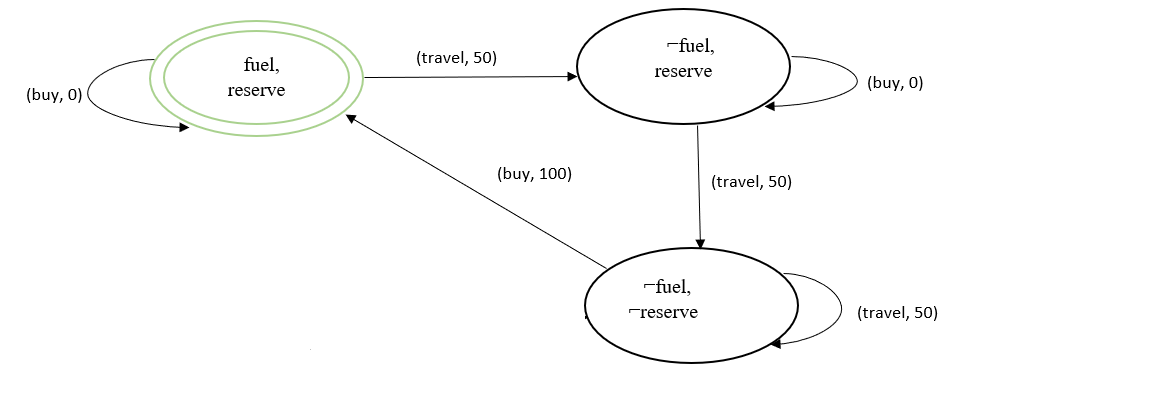
\includegraphics[width=1\linewidth, height=0.3\textheight]{./media/ex01.png}
		\label{Figure:f01}
		\caption{Example 02}
	\end{figure}
	\subsection{Example 02}\label{example:ex02}
	\subsubsection{Description}\label{par:p102}
	John visits a painter to buy a specific painting. The cost of painting is 200$\$$  if its available in the shop. But if painting is not available then John needs to order a new one to be painted that will cost him 100$\$$  extra. At any time only one copy of painting is available and another one to be ordered once sold.
	
	\subsubsection{Representation:}\label{par:p202}
	\indent 
	\par Fluents: available, sold.\par
	Actions: BUY, ORDER.\par
	BUY costs 200$\$$  \textbf{if} available\par
	
	BUY costs 300$\$$  \textbf{after} ORDER\par
	
	
	MIN COST:0$\$$ \par
	
	MAX COST: 300$\$$ \par
	
	
	Always ORDER $\rightarrow$ available\par
	
	Always BUY $\rightarrow$ sold\par
	
	initially: ¬available $\vee$  ¬sold\par
	
	BUY causes sold if available\par
	
	ORDER causes available if ¬available\par
	
	¬available after BUY\\
	
	\subsubsection{Calculation:}\label{par:p302}
	\indent \par
	$ \sum $ = $ \{ $ $ \sigma $ 0, $ \sigma $ 1, $ \sigma $ 2, $ \sigma $ 3$ \} $ \par
	
	$ \sigma $ 0 = $ \{ $ ¬available, ¬sold$ \} $ \par
	
	$ \sigma $ 1 = $ \{ $ ¬available, sold$ \} $ \par
	
	$ \sigma $ 2 = $ \{ $ available, ¬sold$ \} $ \par
	
	$ \sigma $ 3 = $ \{ $ available, sold$ \} $ \par
	\(  \Psi  \)  (BUY, $ \sigma $ 0) = $ \sigma $ 0\par
	
	\(  \Psi  \)  (ORDER, $ \sigma $ 0) = $ \sigma $ 1\par
	
	\(  \Psi  \)  (BUY, $ \sigma $ 1) = $ \sigma $ 2\par
	
	\(  \Psi  \)  (ORDER, $ \sigma $ 1) = $ \sigma $ 1\par
	
	\(  \Psi  \)  (BUY, $ \sigma $ 2) = $ \sigma $ 2\par
	
	\(  \Psi  \)  (ORDER, $ \sigma $ 2) = $ \sigma $ 1\par
	
	\(  \Psi  \)  (BUY, $ \sigma $ 3) = $ \sigma $ 2\par
	
	\(  \Psi  \)  (ORDER, $ \sigma $ 3) = $ \sigma $ 3\par
	\subsubsection{Graph}\label{par:p402}
	\begin{figure}[H]
		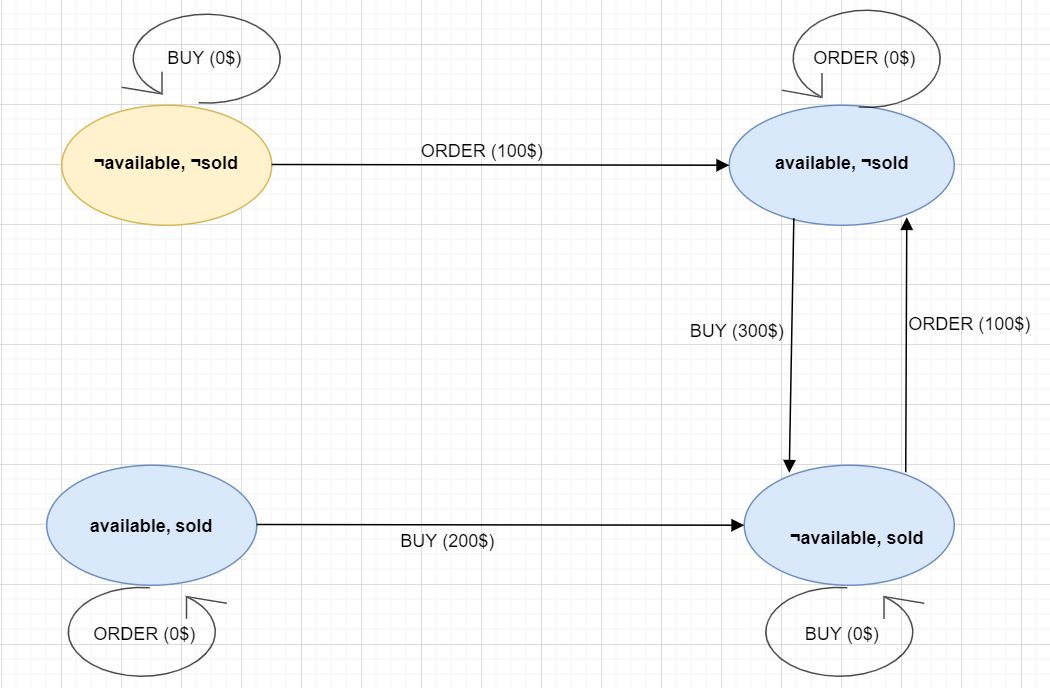
\includegraphics[width=1\linewidth, height=0.3\textheight]{./media/image1.png}
		\label{Figure:f02}
		\caption{Example 02}
	\end{figure}
	\subsection{Example 03}
	\subsubsection{Description}\label{par:p103}
	There is a man. He can cook, eat, and play. Cooking makes food cooked. he can eat food if it is cooked. After eating he feels not hungry, and food is not cooked again. He can play. Playing makes him hungry. He just can play if he is not hungry. He just cooks when there is no food is cooked. Initially, he is hungry, and no food is cooked. In terms of energy, eating costs 5, cooking costs 15, playing costs 20.\\
	\\
	\subsubsection{Representation in language}\label{par:p203}
	Fluents: cooked, hungry.\\
	Actions: cook, eat, play.\\
	\\
	eat cost 5\\
	cooking cost 15\\
	play cost 20\\
	initially $\neg$cooked $\land$ hungry\\
	cook causes cook if $\neg$cooked\\
	eat causes ($\neg$cooked $\land$ $\neg$hungry) if cooked\\
	play causes hungry if $\neg$hungry\\
	\\
	\subsubsection{Calculation}\label{par:p303}
	$\sum$ = \{$\sigma$0 ,$\sigma$1, $\sigma$2, $\sigma$3\}\\
	\\
	$\sigma$0 = \{$\neg$cooked, hungry\}\\
	$\sigma$1 = \{cooked, hungry\}\\
	$\sigma$2 = \{$\neg$cooked, $\neg$hungry\}\\
	$\sigma$3 = \{cooked, $\neg$hungry\}\\
	\\
	$\psi$(eat, $\sigma$0) = $\sigma$0\\
	$\psi$(cook, $\sigma$0) = $\sigma$1\\
	$\psi$(play, $\sigma$0) = $\sigma$0\\
	\\
	$\psi$(eat, $\sigma$1) = $\sigma$2\\
	$\psi$(cook, $\sigma$1) = $\sigma$1\\
	$\psi$(play, $\sigma$1) = $\sigma$1\\
	\\
	$\psi$(eat, $\sigma$2) = $\sigma$2\\
	$\psi$(cook, $\sigma$2) = $\sigma$3\\
	$\psi$(play, $\sigma$2) = $\sigma$1\\
	\\
	$\psi$(eat, $\sigma$3) = $\sigma$2\\
	$\psi$(cook, $\sigma$3) = $\sigma$3\\
	$\psi$(play, $\sigma$3) = $\sigma$1\\
	\\
	\subsubsection{Graph}\label{par:p403}
	\begin{figure}[H]
		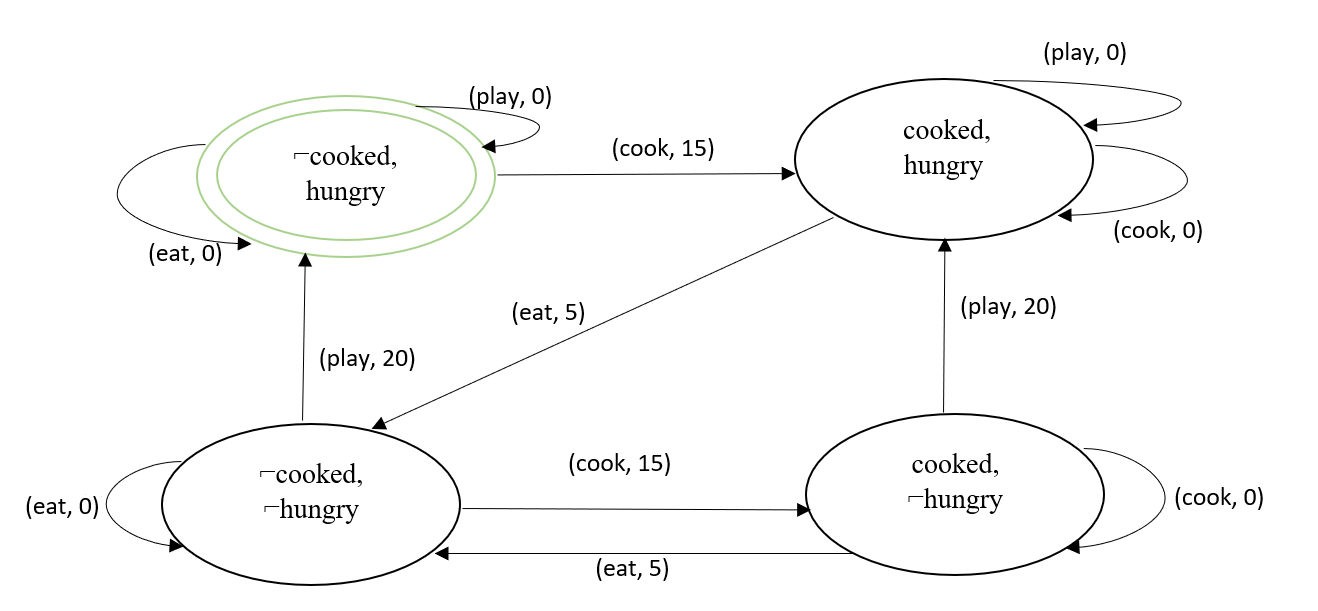
\includegraphics[width=1\linewidth, height=0.3\textheight]{./media/figure01.png}
		\caption{Example 02}
		\label{Figure:f03}
	\end{figure}
	\newpage
	\section{Appendix}	
	\begin{appendix}
		\listoffigures
		\listoftables
	\end{appendix}
\end{document}